% TODO подводку побольше
% QUESTION Этого одного цитирования достаточно на всё?
Генерация с помощью управления атрибутами с использованием архитектуры denoising auto-encoder \cite{lample2018unsupervised, lample2018phrasebased, subramanian2019multipleattribute} является распространённым решением в ситуации отсутствия параллельных данных.
% Естественным решением в ситуации отсутствия параллельных данных является unsupervised подход, который представлен denoising auto-encoder’ом \cite{lample2018unsupervised, lample2018phrasebased, subramanian2019multipleattribute}.

% Основная идея и принципы
% \subsection{Принципы}
% Задача изменения формальности текста является плохо сформулированной задачей, потому что потенциально существует множество способов перефразировать исходное предложение, особенно в неформальный стиль. 
% Тем не менее за последние годы был достигнут впечатляющий прогресс в достижении этой цели и были выделены основные принципы обучения без учителя, как для задачи переноса стиля текста, так и для задачи машинного перевода.

В данном подходе были выработаны три принципа для решения задачи.
Визуализация этих принципов представлена на рисунке \ref{fig:lample_principles}.
На изображении под пунктом A показаны исходные данные: два набора данных, каждый со своим стилем (разные цвета и точки соответствуют предложениям с соответствующим стилем).
Под пунктом Б представлен первый принцип: инициализация. Делается так, чтобы оба распределения примерно совпадали, например, с помощью дословного перевода с использованием словаря.
В пункте В проиллюстрирован второй принцип: языковое моделирование. Языковая модель обучается независимо для каждого стиля для определения структуры данных (изображено в виде непрерывной кривой); она действует как основанная на данных система для устранения шума / исправления предложений (проиллюстрировано пружиной, втягивающей предложение за пределы многообразия обратно).
И, наконец, под пунктом Г изображен третий принцип: обратный перевод (см. \ref{cha:analysis:subsection:backtranslation}).
Начиная с наблюдаемого исходного предложения (заполненный красный круг), используется текущая модель для парафраза (пунктирная стрелка), что приводит к потенциально неправильному переносу стиля (синий крестик рядом с пустым кругом).
Начиная с этого (обратного) перевода, используется модель для переноса стиля в обратную сторону (непрерывная стрелка) для восстановления предложения в оригинальном стиле.
Несоответствие между восстановлением и исходным предложением является сигналом ошибки для обучения параметрам модели.
    Та же процедура применяется в обратном направлении.
\begin{figure}[ht]
  \centering
  \frame{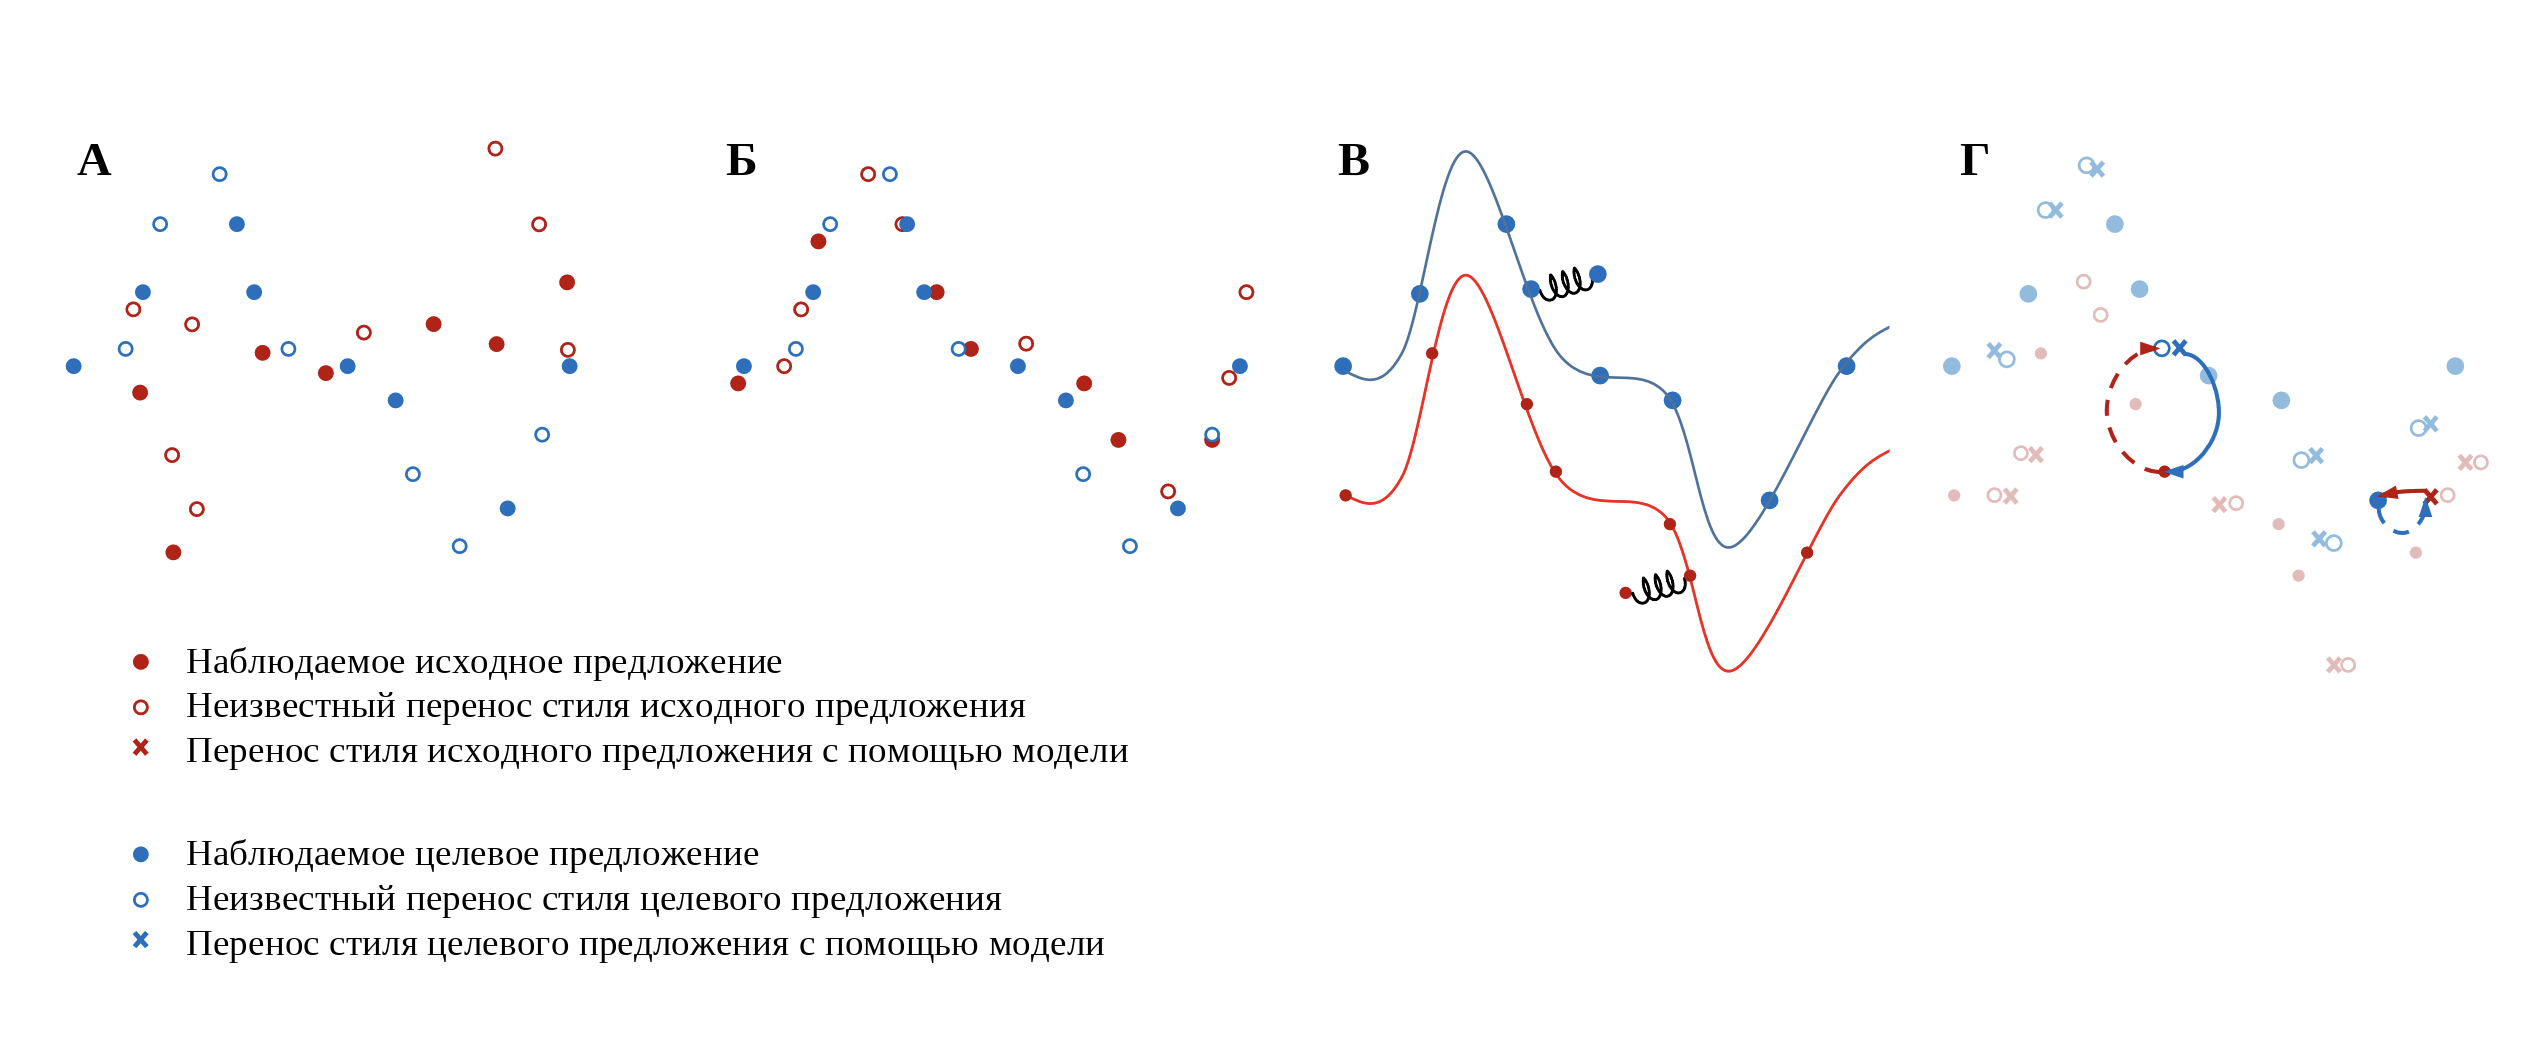
\includegraphics[width=\textwidth]{figures/lample_principles.png}}
  \caption{Принципы алгоритмов "без учителя" для задачи переноса стиля текста}
  \label{fig:lample_principles}
\end{figure}

% Архитектура (в разрезе принципов)
% \subsection{Архитектура модели}
% TODO: overview?
% QUESTION: алгоритм может в виде листинга представить??
% QUESTION: обозначиМ можно? можно в первом лице?
% Листинг алгоритма приведён на рисунке \ref{fig:lample_algorithm}.
% \begin{figure}[ht]
%   \centering
%   \frame{\includegraphics[width=\textwidth]{figures/lample_algorithm.png}}
%   \caption{Алгоритм обучения без учителя для переноса стиля текста}
%   \label{fig:lample_algorithm}
% \end{figure}

% \begin{figure}[ht]
%   \centering
%   \frame{\includegraphics[width=1.0\textwidth]{figures/analysis_lample.png}}
%   \caption{Генерация с помощью управления атрибутами с back-translation}
%   \label{fig:analysis_lample}
% \end{figure}

На этапе инициализации, вместо рассмотрения отдельных слов в предложении, используются byte-pair encoding токены (BPE-токены) \cite{bpe_tokens_article}.
Подобная токенизация даёт два больших преимущества: уменьшает размер словаря и избавляет от присутствия неизвестных UNK-токенов в перефразированном предложении.
BPE-токены обучаются на совместном наборе данных обоих стилей, так как язык одинаковый и большая часть этих токенов будет совпадать. Помимо прочего, в таком случае отпадает необходимость получать словарь между словами разного стиля.
Затем, обучаются word2vec эмбеддинги токенов \cite{mikolov2013distributed}, который затем будут использованы в языковой модели.

% Языковая модель состоит из 
Этап языкового моделирования представлен автокодировщиком с шумоподавлением (denoising autoencoder, DAE) \cite{dae_article, lample2018phrasebased}.
Архитектурой автокодировщика является transformer \cite{attention_is_all_you_need}.
Без каких-либо ограничений обычный автокодировщик очень быстро учится просто копировать каждое вводимое слово одно за другим.
Такая модель также идеально копировала бы последовательности случайных слов, предполагая, что модель не выучивает какую-либо полезную структуру в данных.
Чтобы решить эту проблему, во входные предложения добавляется шум \cite{hill2016learning} и применяется стратегия подавления шума, получая Denoising Autoencoder -- автокодировщик с шумоподавлением \cite{dae_article}.
Общая схема представлена на рисунке \ref{fig:lample_dae}, а функция потерь задаётся как:
$$
\mathcal{L}^{lm} = 
\mathbb{E}_{x \sim \mathcal{S}} [-\log P_{s \rightarrow s}(x|C(x))] +
\mathbb{E}_{y \sim \mathcal{T}} [-\log P_{t \rightarrow t}(y|C(y))]
$$

где $C$ - функция зашумления, которая удаляет или меняет местами некоторые слова \cite{lample2018unsupervised}, а $P_{s \rightarrow s}$ и $P_{t \rightarrow t}$ - композиции энкодера и декодера, оперирующие в исходном или целевом пространстве соответственно.

% QUESTION рассказать подробнее про функцию зашумления?

\begin{figure}[ht]
  \centering
  \frame{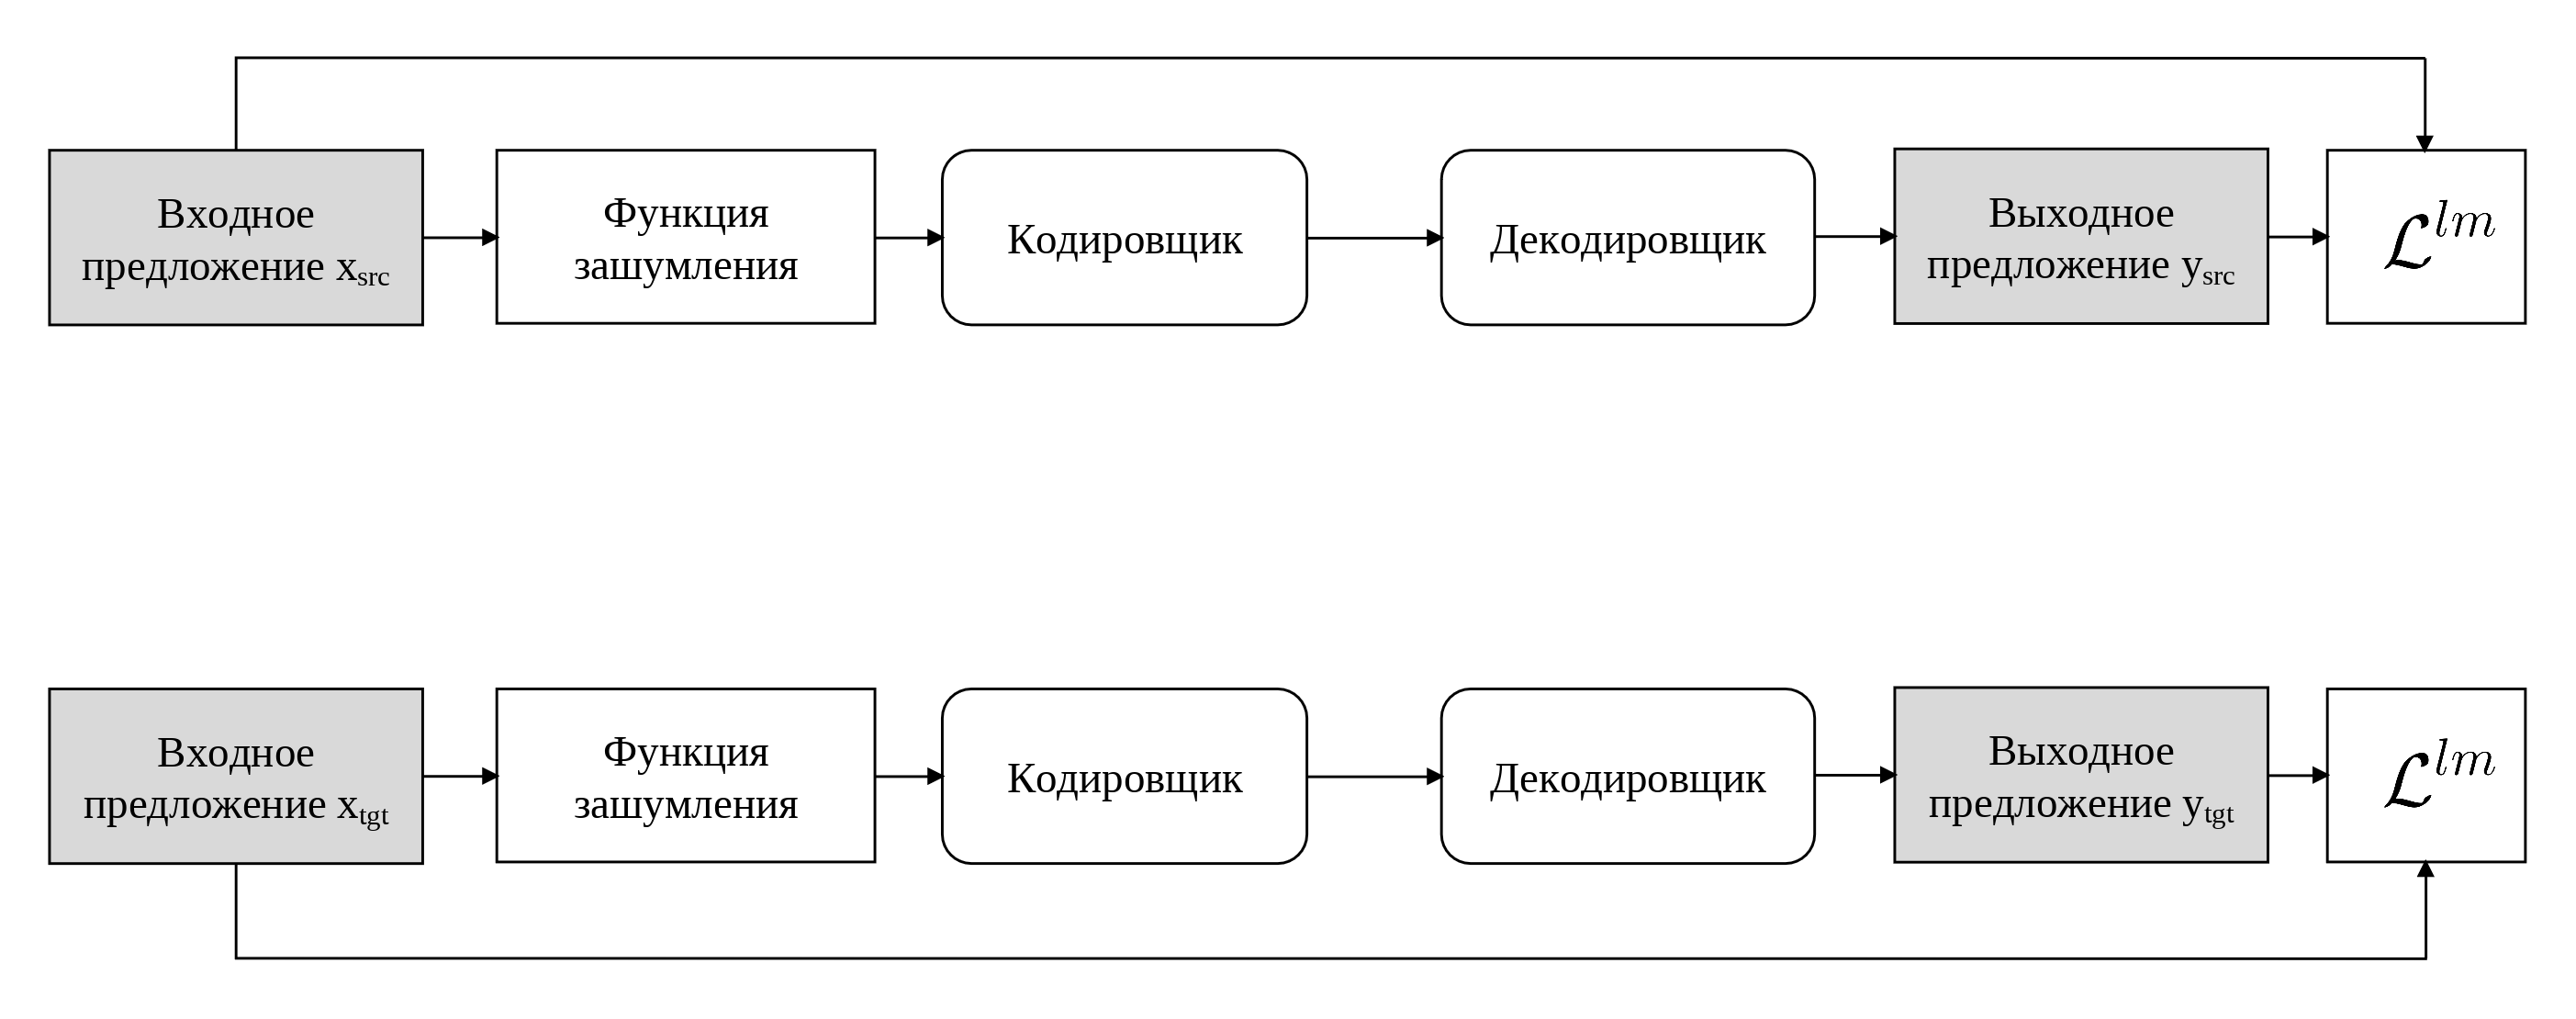
\includegraphics[width=\textwidth]{figures/lample_dae.png}}
  \caption{Обучение denoising auto-encoder}
  \label{fig:lample_dae}
\end{figure}

% Итеративный обратный перевод

% На этом основан механимз back-translation: применим имеющуюся на данную итерацию модель для перевода стиля. Получим парафраз определенного качества. И на полученный парафраз применим обратный перевод: зашумим и пропустим обратно через модель в надежде, что мы сможем восстановить изначальное предложение.

Пространство предложений в исходном и целевом стиле обозначается через $\mathcal{S}$ и $\mathcal{T}$ соответственно, а языковые модели, обученные на исходных и целевых наборах данных, через $P_s$ и $P_t$, соответственно.
Через $P_{s \rightarrow t}$ и $P_{t \rightarrow s}$ обозначим модели парафраза из исходного стиля в целевой и наоборот.
Пусть $u^*(y)$ это предложение в исходном стиле, полученное из $y \in \mathcal{T}$ такое, что $y^*(y) = \arg\max P_{t \rightarrow s}(u|y)$. Подобным образом пусть $v^*(x) = \arg \max P_{s \rightarrow t}(v|x)$.
Таким образом пара $((u^*(y), y)$ и $(x, v^*(x)))$ представляет автоматически перефразированные параллельные предложения, которые могут быть использованы для обучения модели, минимизируя следующую функцию потерь:
$$
\mathcal{L}^{back} = 
\mathbb{E}_{y \sim \mathcal{T}} [-\log P_{s \rightarrow t}(y|u^*(y))] +
\mathbb{E}_{x \sim \mathcal{S}} [-\log P_{t \rightarrow s}(x|v^*(x))]
$$
Этим и выражается третий принцип. Общая схема представленна на рисунке \ref{fig:lample_backtranslation}.

\begin{figure}[ht]
  \centering
  \frame{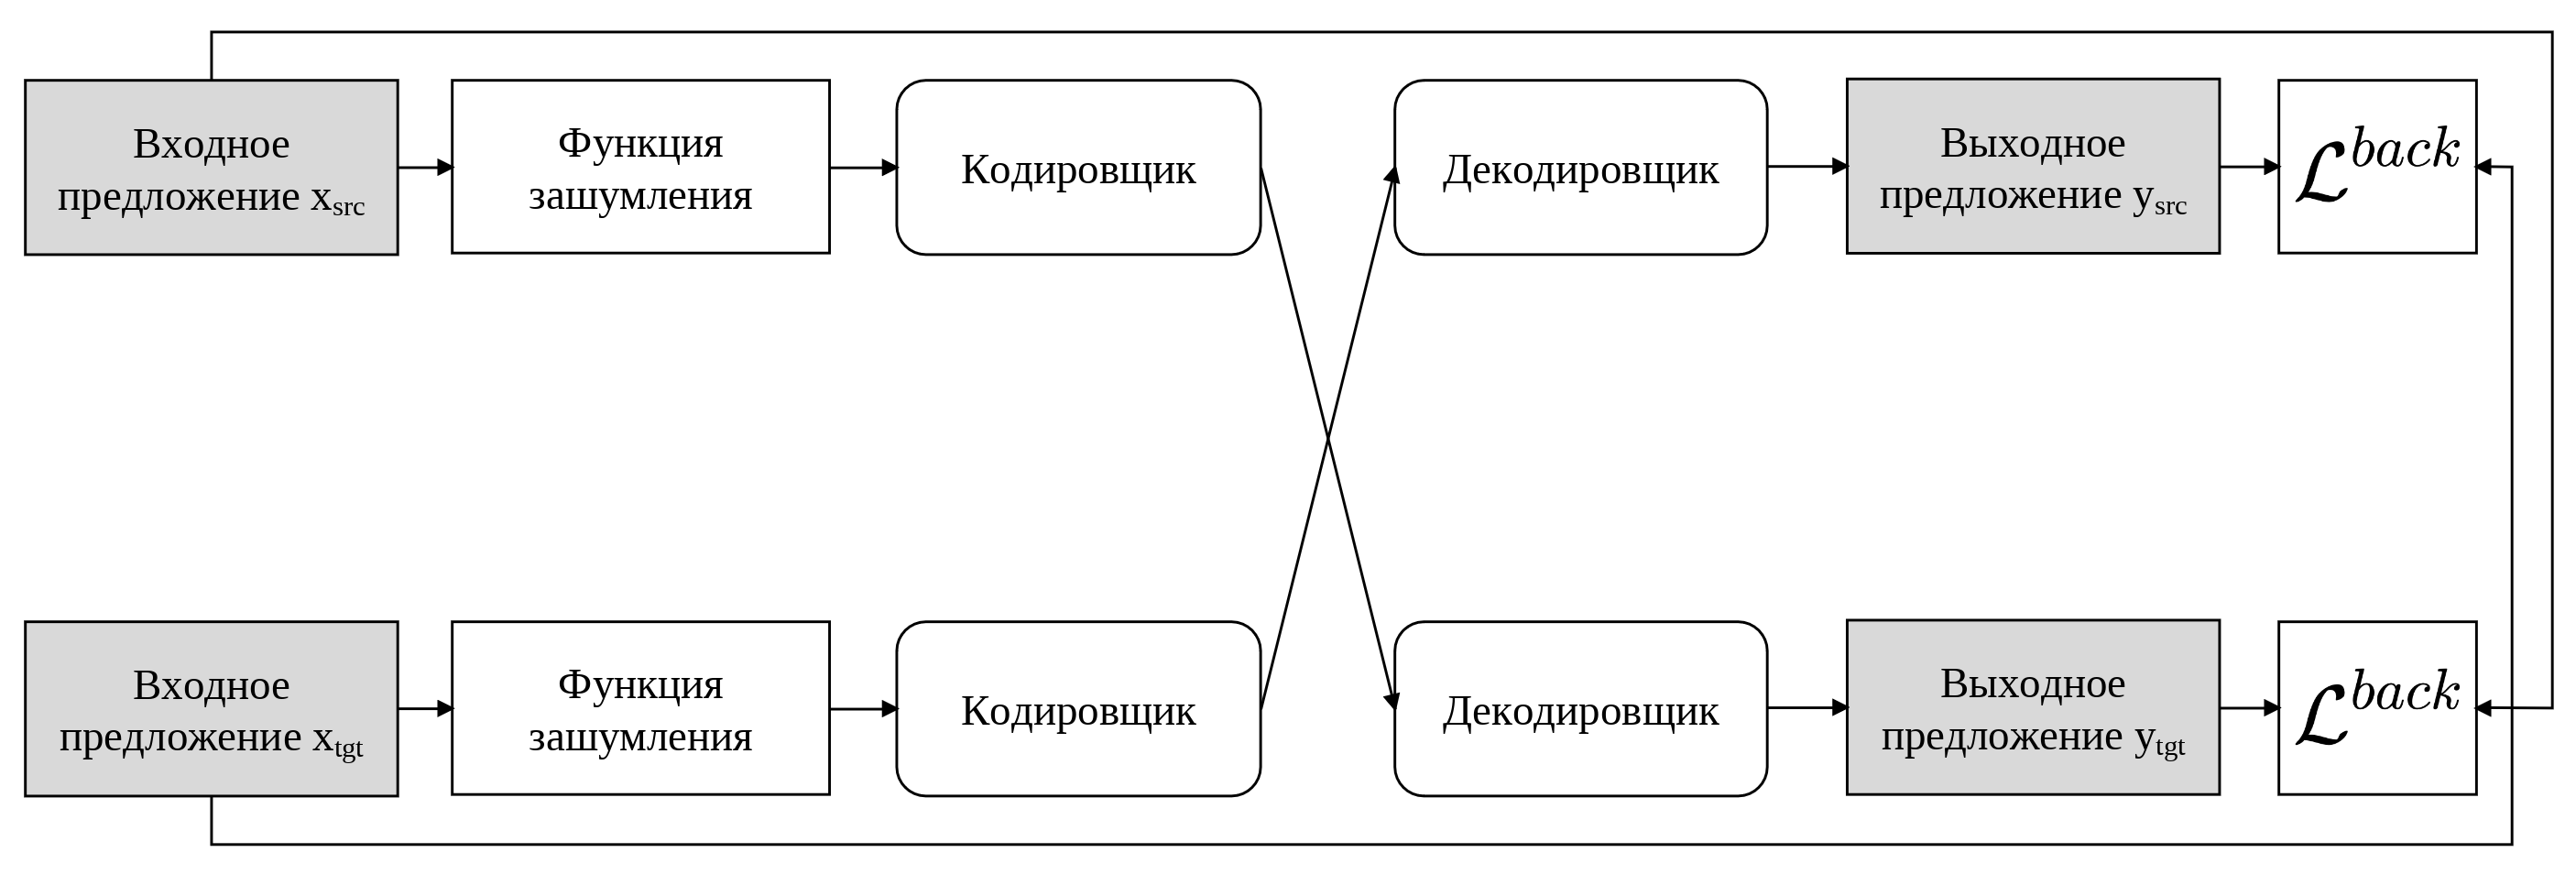
\includegraphics[width=\textwidth]{figures/lample_backtranslation.png}}
  \caption{Обучение с помощью back-translation}
  \label{fig:lample_backtranslation}
\end{figure}

% Он задается 3-мя целевыми функциями:
% \begin{enumerate}
%     \item Это сам авктокодировщик: как хорошо модель может восстановить зашумлённое предложение. Ключевой фактор это функция зашумления, без неё модель будет просто копировать предложения. Здесь эта функция случайным образом удаляла и переставляла местами слова.
%     \item Это функция потерь дискриминатора: дополнительно обучается дискриминатор, который классифицирует исходный стиль эмбеддинга в латентном пространстве. Этот адверсариал-лосс может показаться важным, но на самом деле дальнейшие исследования и мой опыт обучения показывают, что он играет минимальную роль
%     \item И, наконец, третье – самое главное – это кросс-доменная функция потерь. На этом основан механимз back-translation: применим имеющуюся на данную итерацию модель для перевода стиля. Получим парафраз определенного качества. И на полученный парафраз применим обратный перевод: зашумим и пропустим обратно через модель в надежде, что мы сможем восстановить изначальное предложение. Эта кросс-доменная функция потерь измеряет как хорошо это получилось.
% \end{enumerate}

% В качестве модели используется transformer \cite{attention_is_all_you_need}. 
Ключевым параметром является общее использование энкодера между стилями.
Что касается декодера, то авторы заявляют, что его использование оказывает крайне малое влияние \cite{subramanian2019multipleattribute} на качество обучения, однако в рамках данной работы это оказалось ключевым фактором.
Если использовать общий декодер, то модель крайне быстро сходится к тому, что  копирует исходный текст.
Поэтому в итоговой модели используется общий энкодер и два декодера на каждый из стилей.

% Сам процесс обучения итеративный.
% В качестве инициализации используются эмбеддинги fastText и BPE-токенизация. Так как речь идет не о машинном переводе, а о переносе стиля и язык у обоих доменов одинаковый, то эмбединги обучаются совместно. 
% Сначала обучаем определенное количество итераций на задачу денойзинга, получаем первое приближение. Полученную модель копируем и замораживаем и используем для переводов для кросс-доменной функции потерь. После определенного количества итераций, обновляем модель парафраза и повторяем до схождения.

% Во всех методах исследования в качестве монодатасета формального стиля используется случайная подвыборка из википедии по размерам равная имеющемуся монодатасету луркморье




Метрики качества указаны в таблице \ref{table:results}, а примеры генерации в приложении \ref{cha:appendix1}.